\documentclass[12pt,english]{scrartcl}

\usepackage{amsmath,amsfonts,amssymb,amscd,amsthm,amsbsy,alltt,bera,upref,fancyvrb}
\usepackage[T1]{fontenc}
\usepackage{babel}
\usepackage{graphicx}
\usepackage{tikz}

\textheight=10.0truein
\textwidth=6.8truein
\hoffset=-.5truein
\voffset=-.5truein
\pagestyle{headings}
\footskip=36pt
\swapnumbers
\DefineVerbatimEnvironment{code}{Verbatim}{fontsize=\small}
\DefineVerbatimEnvironment{example}{Verbatim}{fontsize=\small}

\usepackage{xcolor}
\definecolor{shade}{RGB}{240,255,255}
\definecolor{nw}{RGB}{255,239,213}

\makeatletter
    \setkomafont{section}{\color{white}%
        \bfseries\Large
        
\begin{tikzpicture}[overlay]
        \draw[fill=black] (0,-2pt) rectangle
        (\linewidth,16.4pt);
        \end{tikzpicture}}
    \setkomafont{subsection}{\color{black}%
        \bfseries\Large
        \begin{tikzpicture}[overlay]
        \draw[fill=white] (0,-2pt) rectangle
        (\linewidth,16.4pt);
        \end{tikzpicture}}

\def\and{%
  \end{tabular}%
  \hskip 1em \@plus.10fil\relax
  \begin{tabular}[t]{c}}
\makeatother
\makeindex

\title{Technical Report: The Austinites}
\author{
  Sheeyla Garcia\\
  \and
  Jesus Hernandez\\
  \and
  Kyle Nicola\\
  \and
  Stephen Ridings\\
  \and
  Carlos Rodriguez\\
  \and
  Mark Sandan\\  
}
\date{ July 10, 2014 }
\begin{document}
\thispagestyle{plain}
\maketitle
\tableofcontents

\begin{figure}[h!]
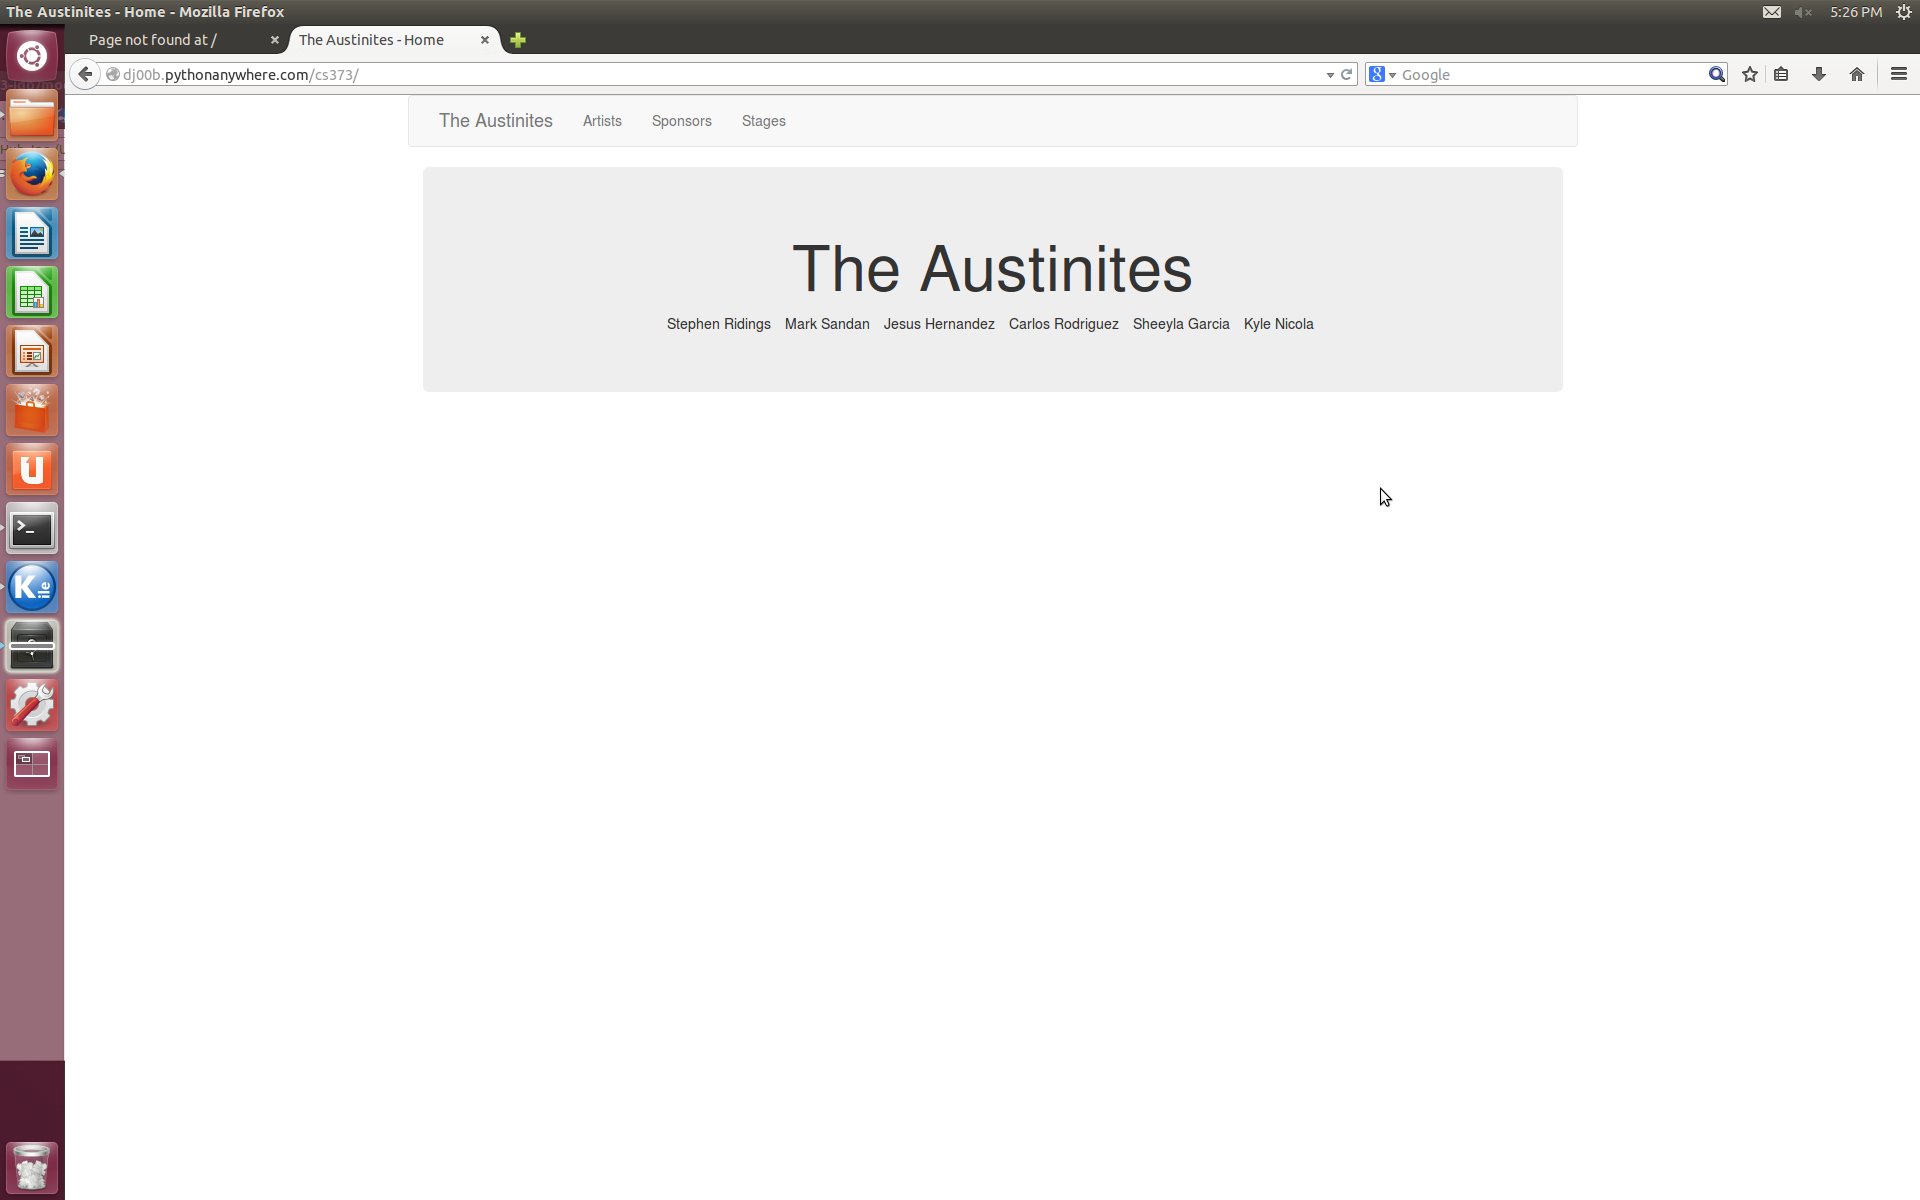
\includegraphics[width=\textwidth]{home}
 \caption{Example Home page showing the group name and the links to the three main pages.}
\end{figure}

\section{Introduction}
The website we are designing is about the 2014 Austin City Limits (ACL) music festival,
 an annual three-day American music festival that takes place on 46-acres in Zilker Park in Austin, Texas. 
The website design has three main pages: Artists, Stages, and Sponsors.
The website allows anyone to view pages about the current Artists, Sponsors, and Stages involved in the festival.
The technologies used are PythonAnywhere, Python 3.4, Django 1.6,
Twitter Bootstrap 3.2, Apiary, and the database sqlite3. PythonAnywhere is used to host the site using the Django web-framework to 
construct the necessary models and views to handle HTTP requests. Twitter Bootstrap is used to organize common data among different
types of pages into a base template HTML file. Apiary is used to provide an API for client-side web access to the information on our webpage.
A problem that we are facing is that the information we need to complete the project hasn't been published as of the date this report
is being written. Currently we are using static HTML pages to stub the relationships betwen HTML pages.

\section{Design}
Our current design of the website uses static HTML pages and Twitter Bootstrap to stylize each page.
Using Django's templating language we are able to reuse html files by extending from them. Currently we only have a single base html page that is extended from and 
uses Twitter Bootstrap. We have nine pages in static HTML that provide examples of the web page design and content. The design and content of each page is outlined below.
\begin{figure}[h!]
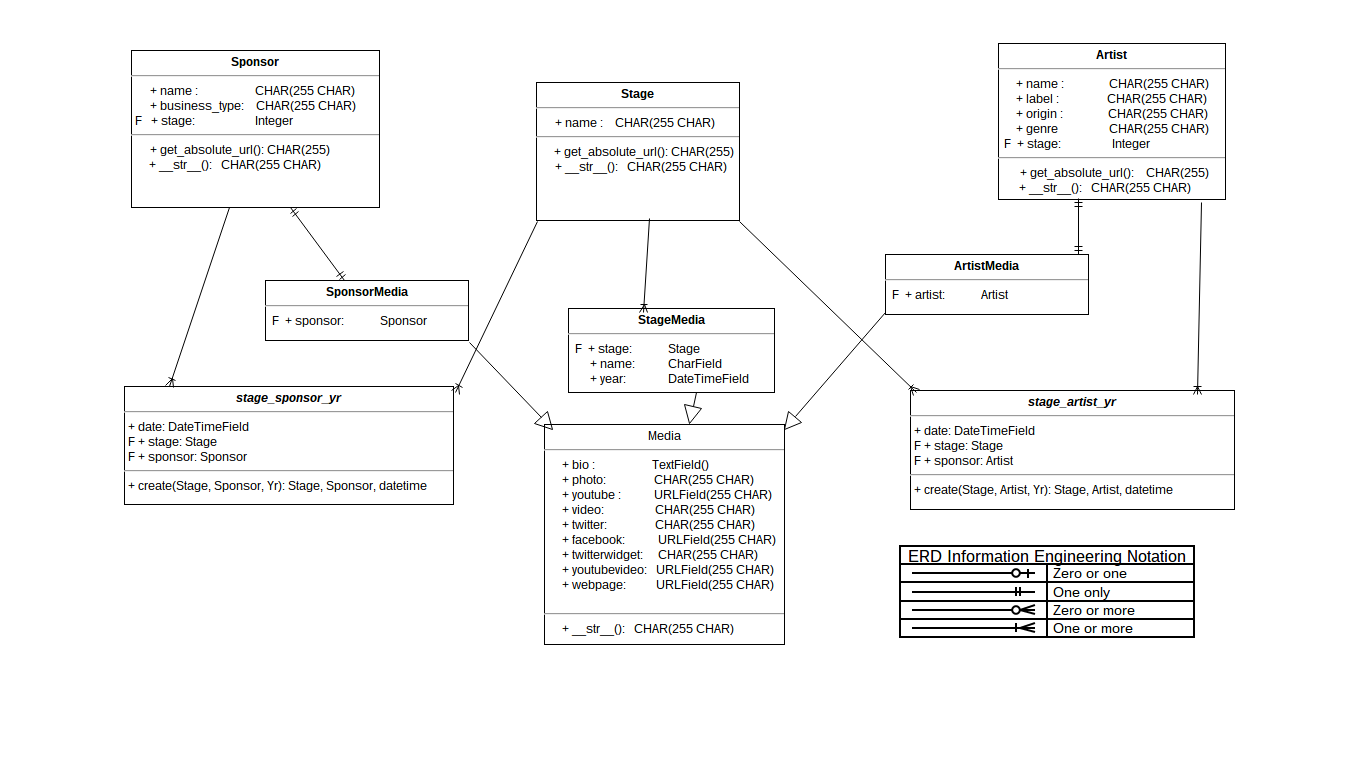
\includegraphics[width=\textwidth]{UML}
 \caption{The current UML schema depicting the relationships between the Django models.}
\end{figure}

\subsection{Web Pages}
Each web page has basic information about a particular artist, sponsor, or stage involved in the ACL music festival.
All pages will include a navigation bar at the top of their page that will allow the user to go back to the main "splash" page, as well as reach the Artists, Sponsors, and
Stages pages. In future phases we are considering incorporating a search bar inside of the navigation bar, so that the user can search
all categories. Mobile browsers are able to view the webpage correctly and set the height and width to a percentage of the size of the screen.

\subsubsection{Splash Page}
\begin{itemize}
 \item Location: https://theaustinites.pythonanywhere.com/
\end{itemize}

The "splash" page will be the first page a visitor to the site will see. It will provide button style links to all subcategories (Artists,
Sponsors, Stages). Currently the page lists the group name and group members.

\subsubsection{Artists}
\begin{itemize}
 \item Location: https://theaustinites.pythonanywhere.com/artists
\end{itemize}

Artist Pages can be reached from the home page as well as from the Stage or Sponsor pages depending on whether the Artist played on
a Stage that was hosted by a Sponsor.The page currently lists the static html pages for music artists Eminem, Pearl Jam, and Outkast

Each Artist page includes the Artist name, an Artist photo, the label, the origin, genre, the sponsor,the stage, a bio,
the official website to the sponsor, a facebook page, a bio, youtube video, youtube channel, and twitter feed.

\subsubsection{Sponsors}
\begin{itemize}
 \item Location: https://theaustinites.pythonanywhere.com/sponsors
\end{itemize}

Sponsor pages can be reached from the home page as well as from the Artist or Stages pages depending on whether the Sponsor hosted a
Stage, and that particular Artist played on that Stage. The page currently lists ACL festival sponsors Honda, Miller Lite, and Samsung Galaxy.

Each Sponsor page includes the Sponsor name, a sponsor logo, the origin, stage sponsored, the artists playing the stage, the official website to the sponsor,
a facebook page, a bio, youtube video, and twitter feed.

\subsubsection{Stages}
\begin{itemize}
 \item Location: https://theaustinites.pythonanywhere.com/stages/
\end{itemize}

Stage pages can be reached from the Home page (splash) as well as from the Artist or Sponsor pages depending on whether the Sponsor hosted a
Stage, and that particular Artist played on that Stage. The page currently lists sponsored stages Honda Stage, Miller Lite Stage, and Samsung Stage.

Each Stage page includes the Stage name, a Stage logo, the artists playing the stage, the official website to the sponsor,
a facebook page, youtube video, and twitter feed.

\subsection{RESTful  API}
The API allows GET requests to the following models: Stages, Sponsors, Artists, Members, and  Photos.
The following section will detail the attributes for the modules, and how the server will respond to the GET requests. See 
the Links section below to view the Apiary API.

\subsubsection{Stages}
When a GET is called on $[/stages]$ it will return a HAL+JSON representation of all the Stages in the database.  It will be a list of the stages along with their attributes.
When a GET is called on $[/stages/{id}]$ it will return a HAL+JSON representation of a single Stage in the database with the given id.  It will list the stage and all of it's attributes
\\
Example of single stage:
\begin{verbatim}
{
         "_links": {
                "self": { "href": "stages/42" }
         },
         "id": 42,
         "name": "Stage name"
}
\end{verbatim}
\subsubsection{Sponsor}
When a GET is called on $[/sponsors]$ it will return a HAL+JSON representation of all the Sponsors in the database.  It will be a list of the sponsors along with their attributes.
When a GET is called on $[/sponsors/{id}]$ it will return a HAL+JSON representation of a single Sponsor in the database with the given id.  It will list the sponsor and all of it's attributes
\\
Example of single sponsor response:
\begin{verbatim}
{
        "_links": {
                "self": { "href": "sponsors/42" }
        },
        "id": 42,
        "name": "Sponsor name",
        "business_type": "Type of Business",
        "website": "URL of sponsor website",
        "stage": 12
}
\end{verbatim}

\subsubsection{Artist}
When a GET is called on $[/artists]$ it will return a HAL+JSON representation of all the Artists in the database.  It will be a list of the artists along with their attributes.
When a GET is called on $[/artists/{id}]$ it will return a HAL+JSON representation of a single Artist in the database with the given id.  It will list the artist and all of it's attributes.
\\
Example of single artist:
\begin{verbatim}
{
        "_links": {
               "self": { "href": "artists/42" }
        },
        "id": 42,
        "name": "Artist name"
        "label": "Label of artist"
        "origin": "Where the artist was from"
        "website": "URL to the artist"
        "genre": "Genre of the artist"
        "stage": 22
}
\end{verbatim}
\subsubsection{Member}
When a GET is called on $[/artists/{artist\_id}/members/]$ it will return a HAL+JSON representation all the Members in the database for the given artist id.  It will be a list of the members along with their attributes.
When a GET is called on $[/artists/{artist\_id}/members/{id}]$ it will return a HAL+JSON representation of a single Member in the database with the given id.  It will list the member and all of it's attributes
\\
Example of single member:
\begin{verbatim}
{
        "_links": {
               "self": { "href": "artists/22/members/42" }
        },
        "id": 42,
        "first_name": "Member's first name"
        "last_name": "Member's last name"
        "artist_id": 22
}
\end{verbatim}
\subsubsection{Photo}
When a GET is called on $[/artists/{artist\_id}/photos/]$ it will return a HAL+JSON representation of all the Photos in the database for the given artist id.  It will be a list of the photos along with their attributes.
When a GET is called on $[/artists/{artist\_id}/photos/{id}]$ it will return a HAL+JSON representation of a single Photo in the database with the given id.  It will list the photo and all of it's attributes
\\
Example of single photo:
\begin{verbatim}
{
        "_links": {
               "self": { "href": "artists/22/photos/42" }
        },
        "id": 42,
        "file_name": "photo.jpg"
        "artist_id": 22
}
\end{verbatim}

\subsection{Django Models}
The Django models created represent the entities we intend to keep in the database for the future when using dynamically loaded pages.
The following subsections document the attributes and intended functionality of each class instance method. The following sections use
$child$ and $parent$ in the sense of the schema relationship depicted by the UML diagram in Figure 2 and not in the sense of the object oriented inheritance 
(the only object each model extends is models.Model). Currently there are a total of five models.

\subsubsection{Artist}
The Artist class represents the current Artists playing on a sponsored stage. All Artists will be a child of some
stage depending on whether they are playing that Stage or not. We are assuming that an Artist will play on 
exactly one stage. The Artist class is implemented using the following:
\begin{verbatim}
attributes:
- id: Primary Key, integer type field.
- name: the name of max length 400 characters.
- label: the artist label with a maximum length of 400 characters.
- origin: the place of origin the artist/group formed with a maximum length of 400 characters.
- website: the official website of the artist or fan site if none. Maximum length of 400 characters.
- genre: the genre associated with the artist. May span more than one. maximum length of 400 characters.
- stage: Foreign Key, integer of type field.

methods:
- get.url(): returns the string "/artists/{id}" . Maximum of number of 400 characters.
- __str__(): returns the name string of the artist.
\end{verbatim}


\subsubsection{Sponsor}
The Sponsor class represents the ACL sponsors that sponsor a Stage for the Artist to perform on.
This relationship is expressed using the one-to-many relationship between the Sponsor and the Stage
class. 

The Sponsor class has the following attributes and methods:
\begin{verbatim}
attributes:
- id: Primary Key, integer type field
- name: a character type field with a maximum length of 400 characters
- business_type: a character type field with a maximum length of 400 characters
- website: a character type field with a maximum length of 400 characters
- stage: Foreign Key, integer of type field

methods:
- get.url(): returns the string "/sponsors/{id}". Maximum number of 400 characters.
- __str__(): returns a string that represents the name of the sponsor.
\end{verbatim}

\subsubsection{Stage}
The Stage class is meant to represent the stage that an Artist will perform on. All stages
have one sponsor. The Stage class extends from the Django models.Models class.

The Stage class has the following attributes and methods:
\begin{verbatim}
attributes:
- id: Primary Key, integer type field
- name: a character type field with a maximum length of 400 characters
- sponsor: Foreign Key, integer of type field

methods:
- get.url(): returns the string "/stages/%s/{name}" where name is the stage name.
- __str__(): returns a string that represents the name of the stage
\end{verbatim}

\subsubsection{Photo}
The Photo class represents a path to a photo of an Artist. 
All Photo's are associated with an Artist in a many-to-one relationship.
This is expressed with the Foreign key being an Artist that the Photo is associated with. 
The Photo class has the following attributes and methods:
\begin{verbatim}
attributes:
-file_name: A CharField of 400 characters. File name of the photo. 
-artist: The ForeignKey relating a Photo to an Artist.

methods:
- __str__(): returns the file_name of the photo.
\end{verbatim}

\subsubsection{Member}
The Member class is meant to represent the members of the Artist group.Thus there is a many-to-one relationship between Member and Artist.
The Member class has the following attributes and methods:
\begin{verbatim}
attributes:
-first_name: A CharField of 400 characters. 
-last_name: A CharField of 400 characters.
-artist: ForeignKey relating the Member to Artist. Integer type field.

methods:
- __str__(): returns the string of form "{first_name} {last_name}" if there is
             a last anme available. Otherwise "{first_name}" is returned.
\end{verbatim}

\section{Unit Tests}
The unit tests currently implemented reflect the expected functionality of the django models and database.
Currently we are using the sqlite3 database as a backend. We assume for each function in the set of tests that the state of the database is reset.
There are currently 30 tests with at least 4 tests for each model. The following give descriptions of each model test. 

\subsection{Stage Test}
Total tests: 7
\begin{itemize}
\item test\_create\_empty\_stage: Tests that uninitialized (stateless) Stages can be created.

\item test\_create\_stage : Tests that the $name$ attribute is set correctly when initialized.
 
\item test\_get\_stage: Tests that the $get\_stage$ method returns the Stage instance we saved into the database. Also tests the filtering functionality of setting the id of the instance.

\item test\_stage\_name: Tests the $max\_length$ property of CharField when setting the name of Stage.

\item test\_stage\_url\_1, test\_stage\_url\_2,test\_stage\_url\_3: Tests whether an instance of the desired Stage class 
is saved in the database table and returns the correct $url$ attribute. 
\end{itemize} 

\subsection{Artist Test}
Total tests: 8
\begin{itemize}
\item test\_create\_artist: Tests the Artist instance attributes actually match the given values
that were passed when constructed (including a Stage instance)
 
\item test\_get\_artist: Tests that an instance of Artist can be retrieved from the database with the attributes used to create it.
 
\item test\_empty\_artist: Tests that an IntegrityError is thrown when an Artist instance is saved in the database without setting a ForeignKey.
 
\item test\_empty\_artist\_with\_stage: Tests the default values of an Artist instance with a ForeignKey.
 
\item test\_artist\_name: Tests the $max\_length$ property of CharField when setting the name of Artist.
 
\item test\_artist\_url\_1, test\_artist\_url\_2, test\_artist\_url\_3: Tests that the many-to-one relationship between
Artists and Stages is valid. Also tests the $get\_url$ method returns the correct url according the id of the instance.
\end{itemize} 

\subsection{Sponsor Test} 
Total tests: 6
\begin{itemize}
\item test\_empty\_sponsor: Tests that a Sponsor's default values and ID are set correctly.
 
\item test\_save\_sponsor: Tests that the name matches the passed value given when the Sponsor instance was created.  
 
\item test\_get\_sponsor\_name: Tests the $max\_length$ property of CharField when setting the name of Sponsor.

\item test\_sponsor\_url\_1, \item test\_sponsor\_url\_2: Tests that the $get\_url$ is returned in the proper format.
\end{itemize}

\subsection{Member Test} 
Total tests: 5

\begin{itemize} 
\item test\_empty\_member:  Tests that a Member can be made with no exceptions when created with an Artist. Tests the default values of Member are empty.
 
\item  test\_get\_empty\_member: asserts that the Member instance is not of type None and that the first\_name attribute is an empty string. 
It also asserts that the Member’s artist attribute is equal to the previously created Artist instance.
 
\item  test\_create\_member: Tests that the attributes are correctly set in Member.
 
\item  test\_get\_member: Tests that the saved Member instance is able to be retrieved from the database and all the values passed 
are correct.
 
\item  test\_str\_member: Tests that the Member string returns the correct $first\_name$ and $last\_name$ of Member.
\end{itemize}

\subsection{Photo Test} 
Total tests: 4
\begin{itemize}
\item test\_empty\_photo: Method is testing whether an instance of Photo is empty.

\item test\_create\_photo: Method is checking that the constructor of the Photo class is working properly when given particular parameters. 

\item test\_get\_photo: Method check the get\_photo method of the Photo class.

\item test\_str\_photo: Method checks the \_\_str\_\_ photo method of the Photo class.
\end{itemize}

\section{Expansions}
This section outlines probable features and functions for the next release.
\begin{itemize}
\item SQLite database to store all information regarding the models and will interact as documented in the RESTful API section

\item HTML pages that utilize the database to work dynamically, as opposed to the static pages currently implemented.

\item More information in the HTML pages such as information on members or link to more social media accounts (Instagram or SoundCloud) for Artist pages.

\item Stage pages will link to a map of the festival so users can see their location.

\item Sponsor models might also include include an attribute to store the location of their headquarters or the name of their respective CEOs.

\item In response to the growth of the models the unit tests will become more robust.

\item  Tests that will check that the database is correctly populated with its new attributes as well as test all the new methods included.

\item An updated API that will include the option to make put requests or delete requests.
\end{itemize}

\section{Links}
\begin{itemize}
 \item Home Page: https://theaustinites.pythonanywhere.com/
 \item Apiary API: http://docs.aclprojectapi.apiary.io/
 \item Github: https://github.com/sandan/cs373-idb
 \item http://www.aclfestival.com/
\end{itemize}

\end{document}